\documentclass[conference]{IEEEtran}

\usepackage{amsmath,amssymb}
\usepackage{booktabs}
\usepackage{graphicx}
\usepackage{cite}
\usepackage{hyperref}
\usepackage{microtype}
\usepackage{multirow}
\usepackage{placeins}
\usepackage{balance}
\usepackage{tikz}
\usetikzlibrary{arrows.meta,positioning,calc,fit,backgrounds}

\hypersetup{hidelinks}
\newcommand{\Huber}{\operatorname{Huber}}
\newcommand{\MAE}{\operatorname{MAE}}

\begin{document}

\title{Compact State-Conditioned NWP Correction with Ensemble Consensus\\
for Multi-Rate Wind Power Forecasting}

\author{
\IEEEauthorblockN{[Authors]}
\IEEEauthorblockA{[Affiliation]}
}

\maketitle

\begin{abstract}
Wind power forecasting combines high-rate historical generation with lower-rate future numerical weather prediction (NWP), yet treating them as symmetric fusion streams can introduce redundant historical modeling and unstable multi-source solutions. We propose a role-separated framework in which a full 6-h power history establishes a baseline trajectory, while the aggregate power trajectory from only the most recent hour conditions a unified NWP correction. For every 15-min target, the correction directly queries all eight native hourly NWP nodes, avoiding explicit weather interpolation. Controlled ablations show that future NWP supplies the dominant correction information, whereas recent power state makes that correction more effective; extending the correction state to the full history gives only a small and seed-unstable improvement. Independently trained correction models nevertheless exhibit substantial prediction diversity. We therefore distill the mean station- and cluster-level predictions of a 10-model ensemble into a student with the same architecture as each teacher member. On the 2023 chronological validation split of a 56-farm, 6.8-GW wind cluster, the resulting single model reduces cluster MAE from 262.1~MW for direct joint forecasting and 258.6~MW for the unstabilized correction model to 251.1~MW. It improves all 10 matched seeds and recovers 53.8\% of the original single-to-ensemble gap without ensemble inference.
\end{abstract}

\begin{IEEEkeywords}
Wind power forecasting, numerical weather prediction, multi-rate forecasting, conditional correction, knowledge distillation
\end{IEEEkeywords}

\section{Introduction}

Short-term wind power forecasting requires two temporally asymmetric signals. Historical generation is observed every 15~min and describes the operating state up to the forecast origin; future numerical weather prediction (NWP) is available at hourly nodes and describes the external forcing over the forecast horizon. The target, however, is again a 15-min trajectory. This is therefore not only heterogeneous feature fusion, but a multi-rate problem: how should coarse-rate future covariates be interpreted from the current generation state to predict a finer-rate response?

Deep forecasting models commonly encode history and future covariates and combine them through concatenation, attention, gating, or feature modulation~\cite{ref_review,ref_attention,ref_tft,ref_film}. Such symmetric fusion is flexible, but obscures the different predictive responsibilities of the inputs. It can also create a second full-history route even after history has already established a forecast trajectory. In wind forecasting, where NWP quality and the current operating regime play distinct roles~\cite{ref_pinson,ref_nwp_nature}, this redundancy complicates both model design and optimization.

Our experiments suggest a more specific allocation of information. With a common full-history baseline, NWP supplies most of the remaining predictive improvement. Additional history is ineffective as a residual predictor by itself, but becomes useful when NWP is present. A frozen-baseline state ladder further shows that current aggregate power, its short trend, and the recent trajectory contribute successively, whereas a second full 6-h correction history gives little beyond the recent hour. These observations motivate
\begin{equation}
    \hat{\mathbf Y}=B(\mathbf H)+C(\mathbf S_{\mathrm{recent}},\mathbf W,\boldsymbol\tau),
    \label{eq:main}
\end{equation}
where the final compact state $\mathbf S_{\mathrm{recent}}$ contains four aggregate 15-min power observations. The correction uses horizon-specific attention over the complete hourly NWP trajectory and is implemented as a general nonlinear mapping. We do not impose a frequency split or claim that its internal weather and state effects are uniquely separable.

The compact correction improves over direct joint forecasting, but its independently trained solutions remain diverse, especially at longer lead times. Their prediction average is substantially stronger than an average member. We therefore use the ensemble mean as a training-only consensus target for an equal-capacity student. This is not model compression from a larger architecture; it regularizes a single model toward a solution shared across optimization runs.

Our contributions are threefold:
\begin{enumerate}
    \item We develop a role-separated multi-rate architecture in which full history supports a baseline, while a compact recent aggregate state conditions a unified correction that directly reads native hourly NWP for each 15-min target.
    \item We provide matched input and state-sufficiency ablations that motivate this allocation. The analysis is used as design evidence rather than presented as the forecasting method itself.
    \item We introduce ensemble-consensus stabilization for the correction model. Same-capacity distillation improves the single model by 7.447~MW over its unstabilized counterpart, with a 95\% paired-seed interval of [6.655, 8.238]~MW and wins on all 10 seeds.
\end{enumerate}

\section{Method}

\subsection{Multi-Rate Forecasting Setup}

Let $N$ be the number of wind farms, $L=24$ the number of historical 15-min steps, and $K=24$ the number of future 15-min targets. Historical station power factors are $\mathbf H\in\mathbb R^{N\times L}$, and the NWP input $\mathbf W$ contains $J=8$ future hourly nodes with 14 meteorological variables on a spatial grid. Station capacities are $a_i$, with total capacity $A=\sum_i a_i$. The compact correction state is the capacity-weighted cluster trajectory over the last four observations,
\begin{equation}
 S_j=\frac{1}{A}\sum_{i=1}^{N}a_i H_{i,j},\qquad
 \mathbf S_{\mathrm{recent}}=(S_{L-3},\ldots,S_L)\in\mathbb R^4.
 \label{eq:state}
\end{equation}
The model predicts station factors $\hat Y_{i,k}$ for leads $\tau_k=k/4$ hours. Cluster power in MW is obtained only after station prediction, $\hat P_k=\sum_i a_i\hat Y_{i,k}$.

\subsection{Baseline and Compact Conditional Correction}

\textbf{Full-history baseline.}
$B(\mathbf H)$ is a history-only model with shared temporal convolutional encoders for station and aggregate power, relative-time history attention, and a temporal residual decoder~\cite{ref_tcn}. It is first trained independently and then used to initialize the baseline in Eq.~\eqref{eq:main}. During final training, $B$ remains trainable. A weak output anchor to the pretrained function $B_0$ discourages arbitrary redistribution between the baseline and correction while retaining joint adaptation.

\textbf{Hourly NWP representation.}
A convolutional weather encoder maps each NWP frame to a spatial feature map. Learned station queries aggregate local grid features and include wind geometry, producing station-specific tokens $\mathbf w_{i,1:J}$. A path encoder represents change across the hourly sequence. For every station $i$ and 15-min horizon $k$, a target token $\mathbf e_{i,k}$ includes station identity, lead time, and forecast-origin phase. Relative-time multi-head attention reads the entire native NWP trajectory,
\begin{equation}
 \mathbf z^W_{i,k}=\operatorname{Attn}\!\left(
 \mathbf e_{i,k},\mathbf w_{i,1:J},\boldsymbol\delta_{k,1:J}\right),
 \label{eq:weatherquery}
\end{equation}
where $\boldsymbol\delta_{k,1:J}$ contains target-to-NWP time offsets. This produces 24 target-specific contexts from eight hourly nodes without deterministic interpolation or NWP super-resolution.

\textbf{Unified correction.}
The four-point aggregate state in Eq.~\eqref{eq:state} is encoded by lightweight temporal encoders. Horizon-specific state responses $\mathbf z^S_{i,k}$ and a global state $\mathbf z^G_k$ are concatenated with the weather and target representations:
\begin{equation}
 C_{i,k}=D_{\theta}\!\left(
 [\mathbf z^S_{i,k},\mathbf z^G_k,\mathbf z^W_{i,k},\mathbf e_{i,k}]
 \right).
 \label{eq:correction}
\end{equation}
$D_\theta$ is a nonlinear response MLP followed by a dilated temporal residual decoder and station output head. The final station prediction is
\begin{equation}
 \hat Y_{i,k}=\left[B_i(\mathbf H)_k+C_{i,k}\right]_+.
\end{equation}
Equation~\eqref{eq:correction} is deliberately a single black-box correction. Explicit additive, multiplicative, FiLM, conditioned-query, attention-bias, and low-rank alternatives did not reliably improve both seed-wise and ensemble criteria. Their components therefore cannot be interpreted as uniquely identified physical effects.

\begin{figure*}[t]
\centering
\resizebox{\textwidth}{!}{%
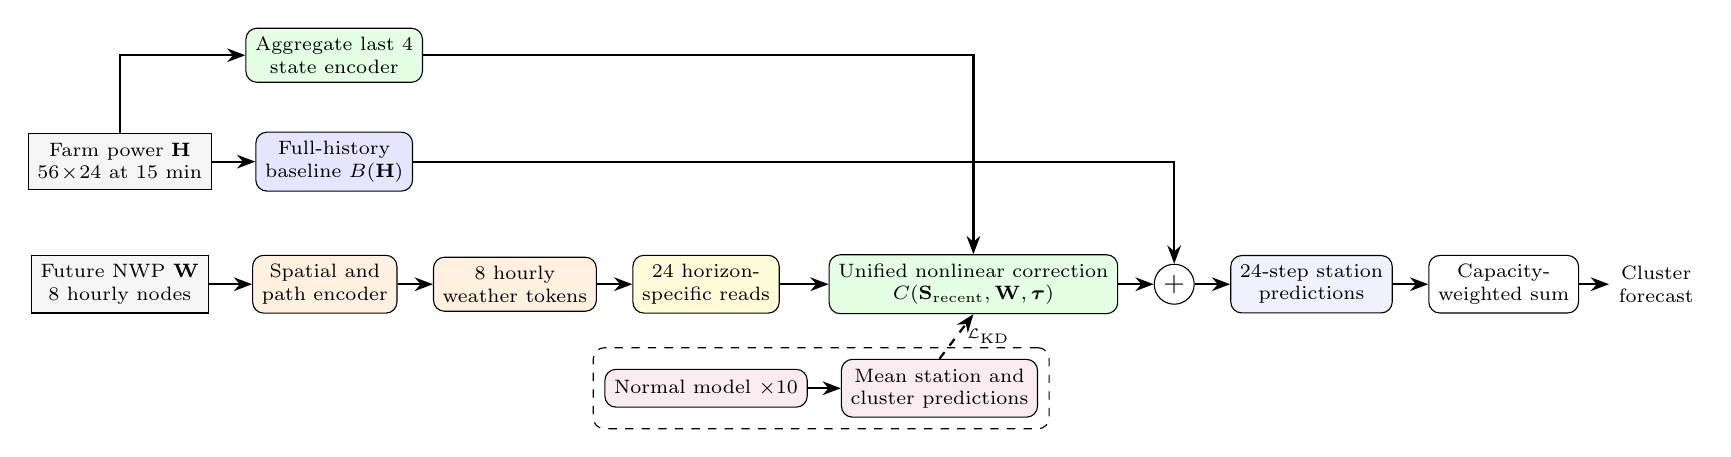
\begin{tikzpicture}[
    >=Stealth,
    node distance=0.38cm and 0.48cm,
    block/.style={draw,rounded corners,minimum height=0.58cm,minimum width=1.55cm,font=\scriptsize,align=center},
    small/.style={draw,rounded corners,minimum height=0.48cm,minimum width=1.25cm,font=\scriptsize,align=center},
    input/.style={draw,minimum height=0.58cm,minimum width=1.55cm,font=\scriptsize,align=center,fill=gray!8},
    line/.style={draw,->,thick},
    train/.style={draw,dashed,rounded corners,inner sep=4pt},
    label/.style={font=\scriptsize,align=center}
]
    \node[input] (hist) {Farm power $\mathbf H$\\$56\!\times\!24$ at 15 min};
    \node[block,right=0.55cm of hist,fill=blue!10] (base) {Full-history\\baseline $B(\mathbf H)$};
    \node[small,above=0.62cm of base,fill=green!10] (state) {Aggregate last 4\\state encoder};

    \node[input,below=0.82cm of hist] (nwp) {Future NWP $\mathbf W$\\8 hourly nodes};
    \node[block,right=0.55cm of nwp,fill=orange!12] (spatial) {Spatial and\\path encoder};
    \node[small,right=0.45cm of spatial,fill=orange!12] (tokens) {8 hourly\\weather tokens};
    \node[small,right=0.45cm of tokens,fill=yellow!15] (query) {24 horizon-\\specific reads};

    \node[block,right=0.62cm of query,fill=green!10] (corr) {Unified nonlinear correction\\$C(\mathbf S_{\rm recent},\mathbf W,\boldsymbol\tau)$};
    \node[draw,circle,right=0.45cm of corr,inner sep=1.5pt] (plus) {$+$};
    \node[block,right=0.45cm of plus,fill=blue!6] (station) {24-step station\\predictions};
    \node[small,right=0.45cm of station] (sum) {Capacity-\\weighted sum};
    \node[label,right=0.38cm of sum] (cluster) {Cluster\\forecast};

    \draw[line] (hist) -- (base);
    \draw[line] (hist.north) |- (state.west);
    \draw[line] (nwp) -- (spatial);
    \draw[line] (spatial) -- (tokens);
    \draw[line] (tokens) -- (query);
    \draw[line] (query) -- (corr);
    \draw[line] (state.east) -| (corr.north);
    \draw[line] (base.east) -| (plus.north);
    \draw[line] (corr) -- (plus);
    \draw[line] (plus) -- (station);
    \draw[line] (station) -- (sum);
    \draw[line] (sum) -- (cluster);

    \node[small,below=0.70cm of query,fill=purple!8] (members) {Normal model $\times 10$};
    \node[small,right=0.42cm of members,fill=purple!8] (teacher) {Mean station and\\cluster predictions};
    \draw[line] (members) -- (teacher);
    \draw[line,dashed] (teacher.north) -- node[right,font=\tiny] {$\mathcal L_{\rm KD}$} (corr.south);
    \node[train,fit=(members)(teacher),label={[font=\tiny]below:training only}] {};
\end{tikzpicture}%
}
\caption{Role-separated multi-rate forecasting and training-only ensemble consensus. Full history supports the baseline; only the last hour of aggregate power enters the correction state. Each 15-min target reads all native hourly NWP tokens. At inference, one student produces station trajectories and the cluster aggregate.}
\label{fig:architecture}
\end{figure*}

\subsection{Ensemble-Consensus Stabilization}

Let $f_{\theta_m}$ denote $M=10$ independently trained instances of the recent-state model~\cite{ref_ensemble}. On training examples $x$, the consensus teacher stores arithmetic-mean station and cluster predictions,
\begin{equation}
 T(x)=\frac{1}{M}\sum_{m=1}^{M} f_{\theta_m}(x).
 \label{eq:teacher}
\end{equation}
A new student $f_\phi$, identical in architecture and parameter count to each member, is optimized by knowledge distillation~\cite{ref_distill} with
\begin{equation}
 \mathcal L=\mathcal L_{\rm sup}
 +\lambda_w\mathcal L_{\rm weather}
 +\lambda_a\mathcal L_{\rm anchor}
 +\lambda_{\rm KD}\mathcal L_{\rm KD},
 \label{eq:loss}
\end{equation}
where $\lambda_w=0.2$, $\lambda_a=0.2$, and $\lambda_{\rm KD}=0.5$. Both $\mathcal L_{\rm sup}$ and $\mathcal L_{\rm KD}$ combine station- and cluster-level Smooth-L1 losses~\cite{ref_huber}, with cluster weight 2; the KD targets include both output levels. $\mathcal L_{\rm weather}$ supervises the auxiliary hourly station weather head, and $\mathcal L_{\rm anchor}$ applies the same station/cluster weighting between $B$ and $B_0$. The teacher is generated only on the training set. The ensemble is thus a training resource, while deployment uses one 1.287-M-parameter student.

\section{Experiments}

\subsection{Setup}

\textbf{Data.}
The dataset contains 56 wind farms in Jilin Province, China, with 6,827~MW total capacity. Power is sampled every 15~min. The NWP fields are hourly Pangu-Weather outputs~\cite{ref_pangu} at $0.25^\circ$ resolution with 14 surface and pressure-level variables. Each origin uses the latest available NWP cycle and eight future nodes. Samples with missing power at any farm are removed rather than interpolated. Models use 2022 for training; all metrics and statistical comparisons reported here use the 2023 chronological validation split, containing 32,550 aligned origins over 359 UTC days. The 2024 split was inspected during earlier development and is therefore neither used here nor claimed as an independent test set. A new temporal or regional holdout remains necessary for final generalization assessment.

\textbf{Protocol.}
All formal groups use matched seeds 42--51. Models have $d=64$ unless marked otherwise, are trained for at most 80 epochs with early stopping, and use identical data processing and optimization budgets. Single-model results are the mean $\pm$ sample standard deviation across 10 seeds. Single-model differences use same-seed paired $t$ intervals. Ensemble and horizon comparisons use 10,000 paired UTC-day block-bootstrap resamples~\cite{ref_bootstrap}. The primary metric is cluster MAE in MW after capacity-weighted aggregation of station forecasts.

\subsection{Main Forecasting Results}

Table~\ref{tab:main} reports the main comparison. Increasing the direct joint model from 0.975 to 1.231~M parameters does not improve its single-model result, while the full-history correction improves it by 3.649~MW with a paired 95\% interval of [2.512, 4.786]~MW and 10/10 seed wins. The compact recent-state model retains similar single-model accuracy: its 258.563~MW is 0.251~MW worse than the full-history correction, but the paired interval [$-0.840$, 1.343] crosses zero. Its ensemble center is reliably 1.816~MW worse [0.476, 3.248]. This is the optimization gap targeted by consensus training.

\begin{table}[t]
\caption{2023 validation cluster MAE (MW), 10 seeds. ``Ens.'' averages the 10 predictions and is diagnostic; the proposed deployment is one KD student.}
\label{tab:main}
\centering
\small
\setlength{\tabcolsep}{3.5pt}
\resizebox{\columnwidth}{!}{%
\begin{tabular}{lccc}
\toprule
Method & Params & Single MAE & Ens. MAE \\
\midrule
History only & 0.975M & 410.471 $\pm$ 0.754 & 407.598 \\
Weather only & 0.975M & 274.231 $\pm$ 1.595 & 260.461 \\
Direct joint, $d=64$ & 0.975M & 262.089 $\pm$ 1.787 & 250.203 \\
Direct joint, $d=72$ & 1.231M & 263.595 $\pm$ 2.024 & 250.038 \\
Full-history correction & 1.287M & 258.311 $\pm$ 1.583 & 242.915 \\
Recent-state correction & 1.287M & 258.563 $\pm$ 1.816 & 244.732 \\
\textbf{Recent state + consensus KD} & 1.287M & \textbf{251.116 $\pm$ 1.617} & \textbf{242.899} \\
\bottomrule
\end{tabular}%
}
\end{table}

Without KD, recent-state correction already improves direct $d=64$ by 3.526~MW [2.236, 4.816] and wins all 10 matched seeds. Consensus KD adds 7.447~MW [6.655, 8.238], again with 10/10 wins, yielding the best single model. The final single model is 10.972~MW better than direct joint forecasting. Its ensemble result is essentially tied with the full-history ensemble, while retaining the compact aggregate correction state.

\subsection{Design Evidence: Information Roles and State Sufficiency}

Table~\ref{tab:design} condenses the design probes. In Panel~A, every cell contains the same trainable full-history baseline and a parameter-matched correction backbone; only the correction input slots are masked. Additional correction history alone changes MAE by just 0.353~MW, with a paired interval crossing zero [$-0.188$, 0.894]. With NWP present, the same input improves MAE by 14.285~MW [12.993, 15.576]. The difference-in-differences is 13.932~MW [12.599, 15.264]. This is predictive evidence for using state to condition the NWP correction, not a physical causal decomposition.

\begin{table*}[t]
\caption{Design probes on 2023 validation (10 seeds). Panel A masks correction inputs while retaining a common full-history baseline. Panel B freezes the same pretrained baseline $B_0$ and varies the state visible to a full-frequency, unified NWP correction.}
\label{tab:design}
\centering
\small
\setlength{\tabcolsep}{6pt}
\begin{tabular}{clcc|clcc}
\toprule
\multicolumn{4}{c|}{\textbf{A. Correction-input roles}} & \multicolumn{4}{c}{\textbf{B. Frozen-baseline state ladder}} \\
 & Correction input & Single MAE & Ens. MAE & & Correction state & Single MAE & Ens. MAE \\
\midrule
1 & context only & 411.962 $\pm$ 0.722 & 408.055 & 1 & weather only & 300.716 $\pm$ 3.300 & 287.404 \\
2 & additional history only & 411.609 $\pm$ 0.799 & 408.304 & 2 & aggregate current & 282.879 $\pm$ 3.500 & 268.894 \\
3 & NWP only & 274.231 $\pm$ 1.595 & 260.461 & 3 & aggregate current + ramp & 270.785 $\pm$ 4.128 & 256.105 \\
4 & additional history + NWP & \textbf{259.946 $\pm$ 1.916} & \textbf{244.229} & 4 & aggregate recent 1 h & 267.214 $\pm$ 3.985 & 252.577 \\
 & & & & 5 & station recent 1 h & 265.759 $\pm$ 3.770 & 250.637 \\
 & & & & 6 & full station history, 6 h & \textbf{264.858 $\pm$ 3.337} & \textbf{249.067} \\
\bottomrule
\end{tabular}
\end{table*}

Panel~B isolates which state is needed by freezing $B_0$. Moving from the current aggregate level to its recent 1-h trajectory improves single-model MAE by 15.665~MW [14.483, 16.848]; a one-step ramp alone does not capture the full benefit. Station-level recent trajectories add a smaller 1.455~MW [0.434, 2.476], whereas extending station recent history to the full 6~h adds only 0.900~MW [$-0.144$, 1.945] and is not seed-stable. The deployed four-point aggregate state is therefore a deliberate compactness--accuracy tradeoff: it preserves the dominant temporal-state gain while avoiding a second $56\times24$ history route. We do not conclude that spatial state is valueless.

The multi-rate read is also empirically motivated. In an earlier three-seed controlled screen, reading the full future NWP path improved ensemble MAE over selecting the nearest hourly node by 4.31~MW, with a paired-day interval of [1.30, 7.08]~MW. Because that comparison has only three seeds, we use it as structural support rather than a headline claim. More elaborate state--weather operators did not provide a stable alternative: for example, Horizon-FiLM improved the black-box ensemble point estimate by 1.110~MW but its seed-wise interval [$-0.375$, 2.590] crossed zero and it significantly degraded the 0.25--1~h band. Conditioned-query and attention-bias variants were no better. The general correction in Eq.~\eqref{eq:correction} is consequently the evidence-based default.

\subsection{Why Consensus Distillation Works}

The unstabilized recent-state models have a 13.831-MW gap between mean single-model MAE and ensemble MAE. Their mean inter-seed prediction disagreement is 103.214~MW and signed-error correlation is 0.8977. Both disagreement and ensemble gain increase with lead time: ensemble gain is 4.081~MW at 0.25--1~h, 11.313~MW at 1.25--3~h, and 18.759~MW at 3.25--6~h. This indicates useful diversity, although the nonnegative pointwise MAE ensemble gain also follows mechanically from convexity and is not itself causal evidence.

\begin{table}[t]
\caption{Single-model stabilization relative to the unstabilized recent-state correction (10 matched seeds). Positive improvement is better.}
\label{tab:stabilization}
\centering
\small
\setlength{\tabcolsep}{3.5pt}
\resizebox{\columnwidth}{!}{%
\begin{tabular}{lccc}
\toprule
Method & Single MAE & Improvement [95\% CI] & Wins \\
\midrule
EMA & 253.494 & 5.069 [3.695, 6.443] & 10/10 \\
Checkpoint average & 256.731 & 1.832 [0.565, 3.098] & 9/10 \\
KD, $\lambda=0.25$ & 254.438 & 4.125 [3.199, 5.050] & 10/10 \\
\textbf{KD, $\lambda=0.5$} & \textbf{251.116} & \textbf{7.447 [6.655, 8.238]} & \textbf{10/10} \\
Uncertainty-aware KD & 252.396 & 6.166 [4.851, 7.481] & 10/10 \\
\bottomrule
\end{tabular}%
}
\end{table}

Table~\ref{tab:stabilization} shows that EMA is a useful low-cost alternative, but plain KD at $\lambda_{\rm KD}=0.5$ is significantly better by 2.378~MW [0.697, 4.058]. KD reduces disagreement from 103.214 to 78.355~MW, increases signed-error correlation to 0.9349, and reduces the model's own single-to-ensemble gap from 13.831 to 8.217~MW. Relative to the original gap, its 7.447-MW single-model improvement corresponds to 53.8\% recovery; the gap itself contracts by 40.6\% because the KD ensemble center also improves. Weighting the teacher inversely by ensemble disagreement is worse than plain KD by 1.280~MW [0.635, 1.926], showing that high member dispersion should not be equated directly with an unreliable ensemble mean.

\FloatBarrier
\balance
\section{Conclusion}

We recast multi-rate wind forecasting as role-separated prediction rather than symmetric source fusion. Full history supports a baseline trajectory; a compact four-point aggregate state conditions a unified correction that queries the complete hourly NWP path for every 15-min target. Input and state-ladder ablations motivate this structure but do not imply a unique physical decomposition. The remaining optimization ambiguity is effectively reduced by training-only ensemble-consensus distillation: the final same-size single model reaches 251.116~MW validation MAE and improves all 10 matched seeds. The evidence currently supports a practical architecture and training mechanism on one cluster, not a universal causal claim. A pristine temporal or regional holdout is the necessary next step before reporting final generalization.

\bibliographystyle{IEEEtran}
\begin{thebibliography}{14}

\bibitem{ref_review}
H.~Wang \textit{et al.}, ``A review of wind speed and wind power forecasting with deep neural networks,'' \textit{Applied Energy}, vol.~304, p.~117766, 2021.

\bibitem{ref_pinson}
P.~Pinson, ``Wind energy: Forecasting challenges for its operational management,'' \textit{Statistical Science}, vol.~28, no.~4, pp.~564--585, 2013.

\bibitem{ref_nwp_nature}
P.~Bauer, A.~Thorpe, and G.~Brunet, ``The quiet revolution of numerical weather prediction,'' \textit{Nature}, vol.~525, pp.~47--55, 2015.

\bibitem{ref_attention}
A.~Vaswani \textit{et al.}, ``Attention is all you need,'' in \textit{Proc. NeurIPS}, 2017.

\bibitem{ref_tft}
B.~N.~Lim \textit{et al.}, ``Temporal fusion transformers for interpretable multi-horizon time series forecasting,'' \textit{International Journal of Forecasting}, vol.~37, no.~4, pp.~1748--1764, 2021.

\bibitem{ref_film}
E.~Perez, F.~Strub, H.~de~Vries, V.~Dumoulin, and A.~Courville, ``FiLM: Visual reasoning with a general conditioning layer,'' in \textit{Proc. AAAI}, 2018.

\bibitem{ref_tcn}
S.~Bai, J.~Z.~Kolter, and V.~Koltun, ``An empirical evaluation of generic convolutional and recurrent networks for sequence modeling,'' \textit{arXiv:1803.01271}, 2018.

\bibitem{ref_pangu}
K.~Bi \textit{et al.}, ``Accurate medium-range global weather forecasting with 3D neural networks,'' \textit{Nature}, vol.~619, pp.~533--538, 2023.

\bibitem{ref_distill}
G.~Hinton, O.~Vinyals, and J.~Dean, ``Distilling the knowledge in a neural network,'' \textit{arXiv:1503.02531}, 2015.

\bibitem{ref_ensemble}
B.~Lakshminarayanan, A.~Pritzel, and C.~Blundell, ``Simple and scalable predictive uncertainty estimation using deep ensembles,'' in \textit{Proc. NeurIPS}, 2017.

\bibitem{ref_bootstrap}
S.~N.~Lahiri, \textit{Resampling Methods for Dependent Data}. Springer, 2003.

\bibitem{ref_huber}
P.~J.~Huber, ``Robust estimation of a location parameter,'' \textit{Annals of Mathematical Statistics}, vol.~35, no.~1, pp.~73--101, 1964.

\end{thebibliography}

\end{document}
